\chapter{Performance Specifications}

The purpose of this lab is to give you an understanding of the performance of
a second-order system.  In particular, you will be examining the effects that
system parameters have on various features of the output of that system.  In
the second part of the lab, you will examine the disturbance type of several
systems.

\section{Prelab}

Before you go into the lab, you should read the following:
\begin{itemize}
    \item Sections 8.2.2, 8.2.3, and 8.3.1 in the course notes on performance specifications.
    \item Be sure to familiarize yourself with the concept of system types.
\end{itemize}
Then, determine the state space representation
\((\mat{A},\vect{b},\vect{c}^{t},\mat{D}) \) of the generic second order model:
\begin{equation*}
    \ddot y +2\zeta\omega_{0}\dot y+\omega_{0}^{2}y=\omega_{0}^{2}u.
\end{equation*}
Next, solve the above differential equation with a step response (\(u = 1\)),
and comment on the effect of \(\zeta \) and \(\omega_0 \), and how this relates to
the location of the poles of your transfer function.

\section{Key Concepts}

\begin{enumerate}
    \item The main idea behind this lab is to understand how the addition of a zero
          affects the response of a system. For your system, let's say you add a zero at the
          point \(\alpha \). What this will do to your governing equation is add a scaled derivative
          of the step response. The derivative of the step response (i.e.\ the impulse response)
          will be scaled by a factor of \(\frac{\omega_0}{\alpha} \). Thus, for very large alpha,
          this term will have little impact on the systems response. However, if this zero exists
          very close to the imaginary axis, your system will have what is called undershoot.
    \item Secondly, you must understand the definition of system types. Essentially,
          systems can be type 0, 1, 2, etc \ldots A systems ``type'' determines its ability to track
          the error on a given reference trajectory. For example, a system of type \(k \) can track
          a reference trajectory with a bounded error for polynomials up to degree \(k \). See Proposition
          8.11 from the course notes for further clarification.


\end{enumerate}

\section{Procedure}

\subsection{Simulation of a second-order system}\label{subsec:simulation}

The model we will be examining is the generic second-order equation, where
the output of the system is position:
\begin{equation}\label{eq:sys}
    \ddot y +2\zeta\omega_{0}\dot y+\omega_{0}^{2}y = \omega_{0}^{2}u.
\end{equation}
Since the physical constants of our friendly motor system cannot be changed
in the simple open-loop configuration, we are confined to the world of
simulations.  We will examine the behaviour of the second-order system in
\textsf{Simulink}.
\begin{enumerate}
    \item Find the poles of your generic second-order system (or eigenvalues of your \(\mat{A} \) matrix).
    \item Open \textsf{Matlab} and build a \textsf{Simulink} model according to
          Figure~\ref{fig:model7}\@.
          \begin{figure}[htbp]
              \centering
              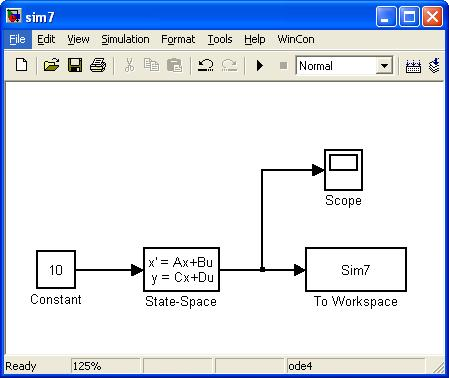
\includegraphics[width=0.6\hsize]{pix/model7.jpg}
              \caption{\textsf{Simulink} model for a generic second-order system}\label{fig:model7}
          \end{figure}%
          You should have determined the values for
          \((\mat{A},\vect{b},\vect{c}^{t},\mat{D}) \) in your prelab. Define these matrices, in terms of \(\zeta \) and \(\omega_{0} \), in a script and simply call them in your model. We will use this model in Section~\ref{NMP}.

    \item Run the system in simulation with initial values of \(\zeta=0.5 \) and
          \(\omega_{0}=1\). As this is a simulation, you do not need to build your system.

    \item Using the \verb|step()| function in Matlab (and a \verb|for| loop), plot several values of \(\zeta \) on the same graph using your \((\mat{A},\vect{b},\vect{c}^{t},\mat{D}) \) matrices.
          Print out the graph and write down your observations related to the response characteristics. It may be helpful to use different style of
          lines for various values of \(\zeta \). Details on plotting with various line
          styles are discussed in Appendix~\ref{chap:MATLAB}\@.

    \item Repeat the previous step with various values of \(\omega_{0}\).
\end{enumerate}

\subsection{Non-minimum phase systems}\label{NMP}

The system described in Section~\ref{subsec:simulation} has the transfer
function
\begin{equation*}
    T(s)=\frac{\omega_{0}^{2}}{s^{2}+2\zeta\omega_{0}s+\omega_{0}^{2}}.
\end{equation*}
We add a zero to the system as follows:
\begin{equation*}
    T(s)=\frac{\hat y(s)}{\hat u(s)}=
    \frac{\omega_{0}^{2}}{s^{2}+2\zeta\omega_{0}s+
        \omega_{0}^{2}}\frac{(s+\alpha)}{\alpha}.
\end{equation*}
We use the parameter \(\alpha \) to vary the position of the zero.  In
particular, we can use it to place our zero in \(\mathbb{R}_{<0} \) or
\(\mathbb{R}_{>0}\).  Notice that we have \(\alpha \) in the denominator as
well.  This is a done to normalize the system at \(s=0\).

To convert this back into the time domain, we simply cross-multiply the
transfer function to get the state equation
\begin{equation*}
    \ddot y +2\zeta\omega_{0}\dot y+\omega_{0}^{2}y =
    \frac{\omega_{0}^{2}}{\alpha}\dot u+\omega_{0}^{2}u.
\end{equation*}
You can see that the only difference is that we now have a term involving
\(\dot u \).  Since \(u \) is a step function, \(\dot{u} \) is going to be an impulse
function.\footnote{The derivative here is understood in the sense of
    distributions.}  Implementing an impulse function cannot be done directly,
but we can side-step the problem by cooking the initial conditions so that
our initial value problem is a solution to our system when given a step
input.  It turns out that these initial conditions are \(y(0)=0 \), and \(\dot{y}(0)=\frac{\omega_{0}^{2}}{\alpha}\).\footnote{This is a little involved,
    but see Section 3.6.5 of the course text for
    details.}
\begin{enumerate}
    \item Modify the model from the previous section to incorporate the zero
          added to the system by adding the initial conditions. The way to enter
          initial conditions into the model is shown in
          Lab~\ref{chap:controlandobserve}.

    \item For \(\alpha = \left\{0.1, 1, 10\right\} \), what is the effect of increasing %chktex 21
          \(\alpha \) on the rise time, settling time, overshoot, and peak
          time?  Using \textsf{Matlab}, plot the output of these positive
          \(\alpha \) values and print the graph.  On the graph, write down your
          discoveries.\label{step1}

    \item For \(\alpha = \left\{-0.1, -1, -10\right\} \), what is the effect of increasing the %chktex 21
          magnitude of \(\alpha \) on the rise time, settling time, overshoot,
          and peak time? Using \textsf{Matlab}, plot the output of these negative \(\alpha \) values and print the graph.  On the graph, write down
          your discoveries.  What is the most noticeable characteristic of a
          non-minimum phase system?\label{step2}
    \item\label{step:superposition} Lastly, we will be observing exactly what the addition of a zero does
          to the system.
          \begin{enumerate}
              \item In Matlab, plot the step response and impulse response of your
                    original system (without the zero) shown in equation~\ref{eq:sys} using the \verb|step| and
                    \verb|impulse| commands.
              \item\label{step3} On a separate graph, plot the addition of the step response with
                    the impulse response scaled by a factor of \(\frac{\omega_0^2}{\alpha} \) (use the same \(\alpha \) values from above). Note: only the impulse response should be scaled. When using the
                    \verb|step| and \verb|impulse| commands, you must ensure that the arrays have the same length in
                    order to superimpose them. This may involve truncating one array to match the length of the other.
              \item Comment on your plots obtained in part~\ref{step3} with those obtained in step~\ref{step1} and~\ref{step2}. Hint: The plots should be the exact same. Comment on why that is.
          \end{enumerate}
\end{enumerate}

\subsection{System type}

We will now examine three different motor system and the system type of each
one.  The basic configuration is shown in
Figure~\ref{fig:feebackWithDisturbance}\@.
\begin{figure}[htbp]
    \centering
    \begin{picture}(240,75)
        \put(0,50){\(\hat\theta_{d}(s)\)}
        \put(20,53){\vector(1,0){15}}
        \put(40,53){\circle{7}}
        \put(45,53){\vector(1,0){15}}
        \put(63,37){\framebox(35,33){\(R_{C}(s)\)}}
        \put(100,53){\vector(1,0){20}}
        \put(123,37){\framebox(80,33){\(R_{P}(s)=\frac{k_{E}}{s(s+\frac{1}{\tau})}\)}}
        \put(205,53){\vector(1,0){30}}
        \put(237,50){\(\hat\theta(s)\)}
        \put(215,53){\line(0,-1){45}}
        \put(215,8){\line(-1,0){175}}
        \put(40,8){\vector(0,1){40}}
        \put(30,48){\line (1,0) {4}}
    \end{picture}
    \caption{Feedback system with disturbance}\label{fig:feebackWithDisturbance}
\end{figure}%
This is an interconnected system, but we will take a ``black box'' approach,
applying the disturbance at the input node, and measuring at the output node.
Recall that the motor is modelled by transfer function
\(\frac{k_{E}}{s(s+\frac{1}{\tau})} \) when the output is the motor angle
\(\theta \).
\begin{enumerate}
    \item System 1 has the controller transfer function \(R_{C}(s)=5\).
          Verify by hand that the transfer function
          \begin{equation*}
              T(s)= \frac{R_{C}(s)R_{P}(s)}{1+R_{C}(s)R_{P}(s)}
          \end{equation*}
          is BIBO stable. Hint: What is \(R_{C} = 5 \) equivalent to? What do we know about this from lab 3?

    \item Determine the system type for this particular system.

    \item Assemble (or modify an existing) a \textsf{Simulink} model according to
          Figure~\ref{fig:model7a}\@.
          \begin{figure}[htbp]
              \centering
              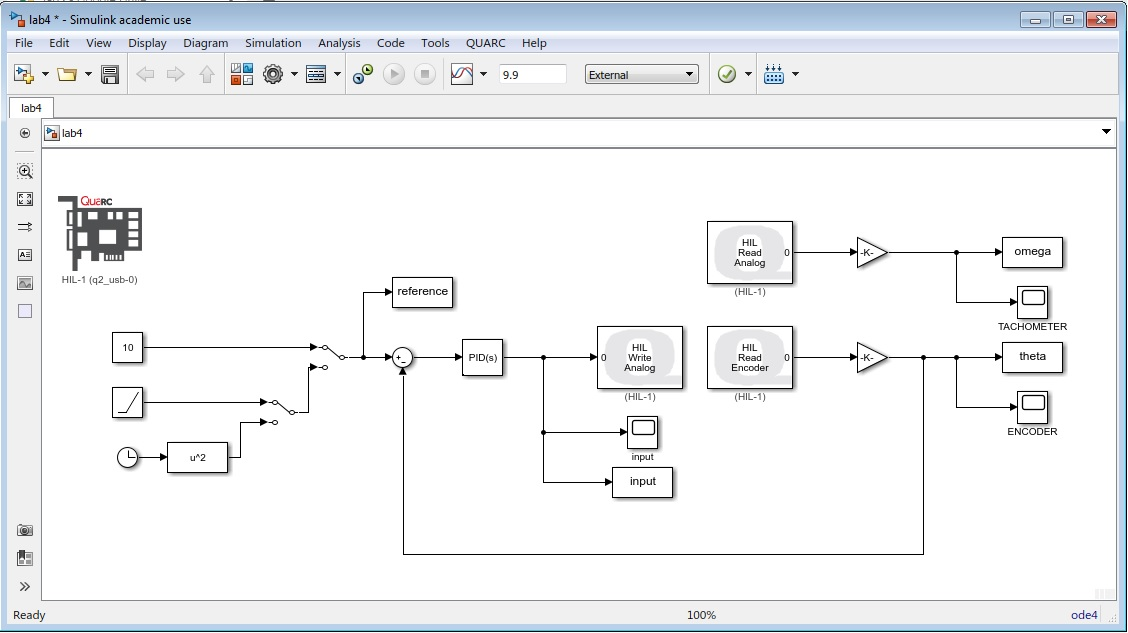
\includegraphics[width=0.6\hsize]{pix/performanceSpecificationModel4.jpg}
              \caption{\textsf{Simulink} model for a DC Servo Motor
                  system}\label{fig:model7a}
          \end{figure}%

    \item Run the system using the constant input.  What is the steady-state
          error of the system?  Plot the error response in \textsf{Matlab} and print a
          copy of the plot with appropriate titles and axis labels. Is this consistent
          with your earlier work?

    \item Repeat the above step, but use a linear and quadratic term (divide the quadratic term by 2 to ensure the encoder does not go out of range) for the
          reference signal.  Plot all the error responses and make print outs.  Make
          sure you have proper axis labels and titles.

    \item System 2 has the same plant transfer function and a new
          controller transfer function given by \(R_{C}(s)=\frac{1}{s}\).  Is this
          system BIBO stable?  If so, what is the system type?

    \item Make changes to the system to implement the new controller and run the
          system with a constant, a linear, and a quadratic reference signal.  Are the
          results consistent with your answer from above?

    \item System 3 has the same plant transfer function and a new
          controller transfer function given by \(R_{C}(s)=s\).  Is this system BIBO
          stable?  If so, what is the system type?

    \item Make changes to the system to implement the new controller and run the
          system with a constant, a linear, and a quadratic reference signal.  Are the
          results consistent with your answer from above?

    \item Plot all the error responses in \textsf{Matlab} graph and print them.
          Make sure you have proper axis labels and titles.
\end{enumerate}

When you have completed the lab, make sure you save your files in the folder
you created in Lab~\ref{chap:intro}\@.

\section{Deliverables}

Prepare a brief write up describing what you learned from this lab. This does not
need to be a formal report, but all material should be presented in a clear and logical manner,
with concise descriptions where necessary. Include the following/Answer the following questions:
\begin{enumerate}
    \item Include plots of the systems response with varying \(\zeta \) and \(\omega_0 \) values, comment
          on the effect off varying these constants.
    \item For both positive and negative \(\alpha \) values, what is the effect of increasing the magnitude
          of \(\alpha \) on the rise time, settling time, overshoot/undershoot, and peak time? Include plots.
    \item In step~\ref{step:superposition} of the non-minimum phase system section, explain why your two
          plots are the same.
    \item Create the following table for the system type section. Be sure to include and reference all
          necessary plots for the justification section.
          \begin{table}[htbp]\label{tab:systype}
              \centering
              \begin{tabularx}{.9\linewidth}{|c|X|X|X|c|c|}\hline %chktex 44
                  System No. & \raggedright{Response to Constant Input} & \raggedright{Response to Ramp Input} & \raggedright{Response to Quadratic Input} &
                  Type?      & Justification                                                                                                                     \\\hline %chktex 44
                  System 1   &                                          &                                      &                                           &   & \\\hline %chktex 44
                  System 2   &                                          &                                      &                                           &   & \\\hline %chktex 44
                  System 3   &                                          &                                      &                                           &   & \\
                  \hline %chktex 44
              \end{tabularx}
          \end{table}
\end{enumerate}

%%% Local Variables: 
%%% mode: latex
%%% TeX-master: "lab-manual"
%%% End: 
